\chapter{Conic Sections}

In mathematics, conic sections (or simply conics) are curves obtained
as the intersection of the surface of a cone with a plane. The three
types of conic section are the hyperbola, the parabola, and the
ellipse. The circle is a special case of the ellipse, though
historically it was sometimes called a fourth type. All of the equations below can be graphed on programs like Desmos. \index{conic sections}

\begin{center}
    

\end{center}

\begin{figure}[htbp]
  \centering
  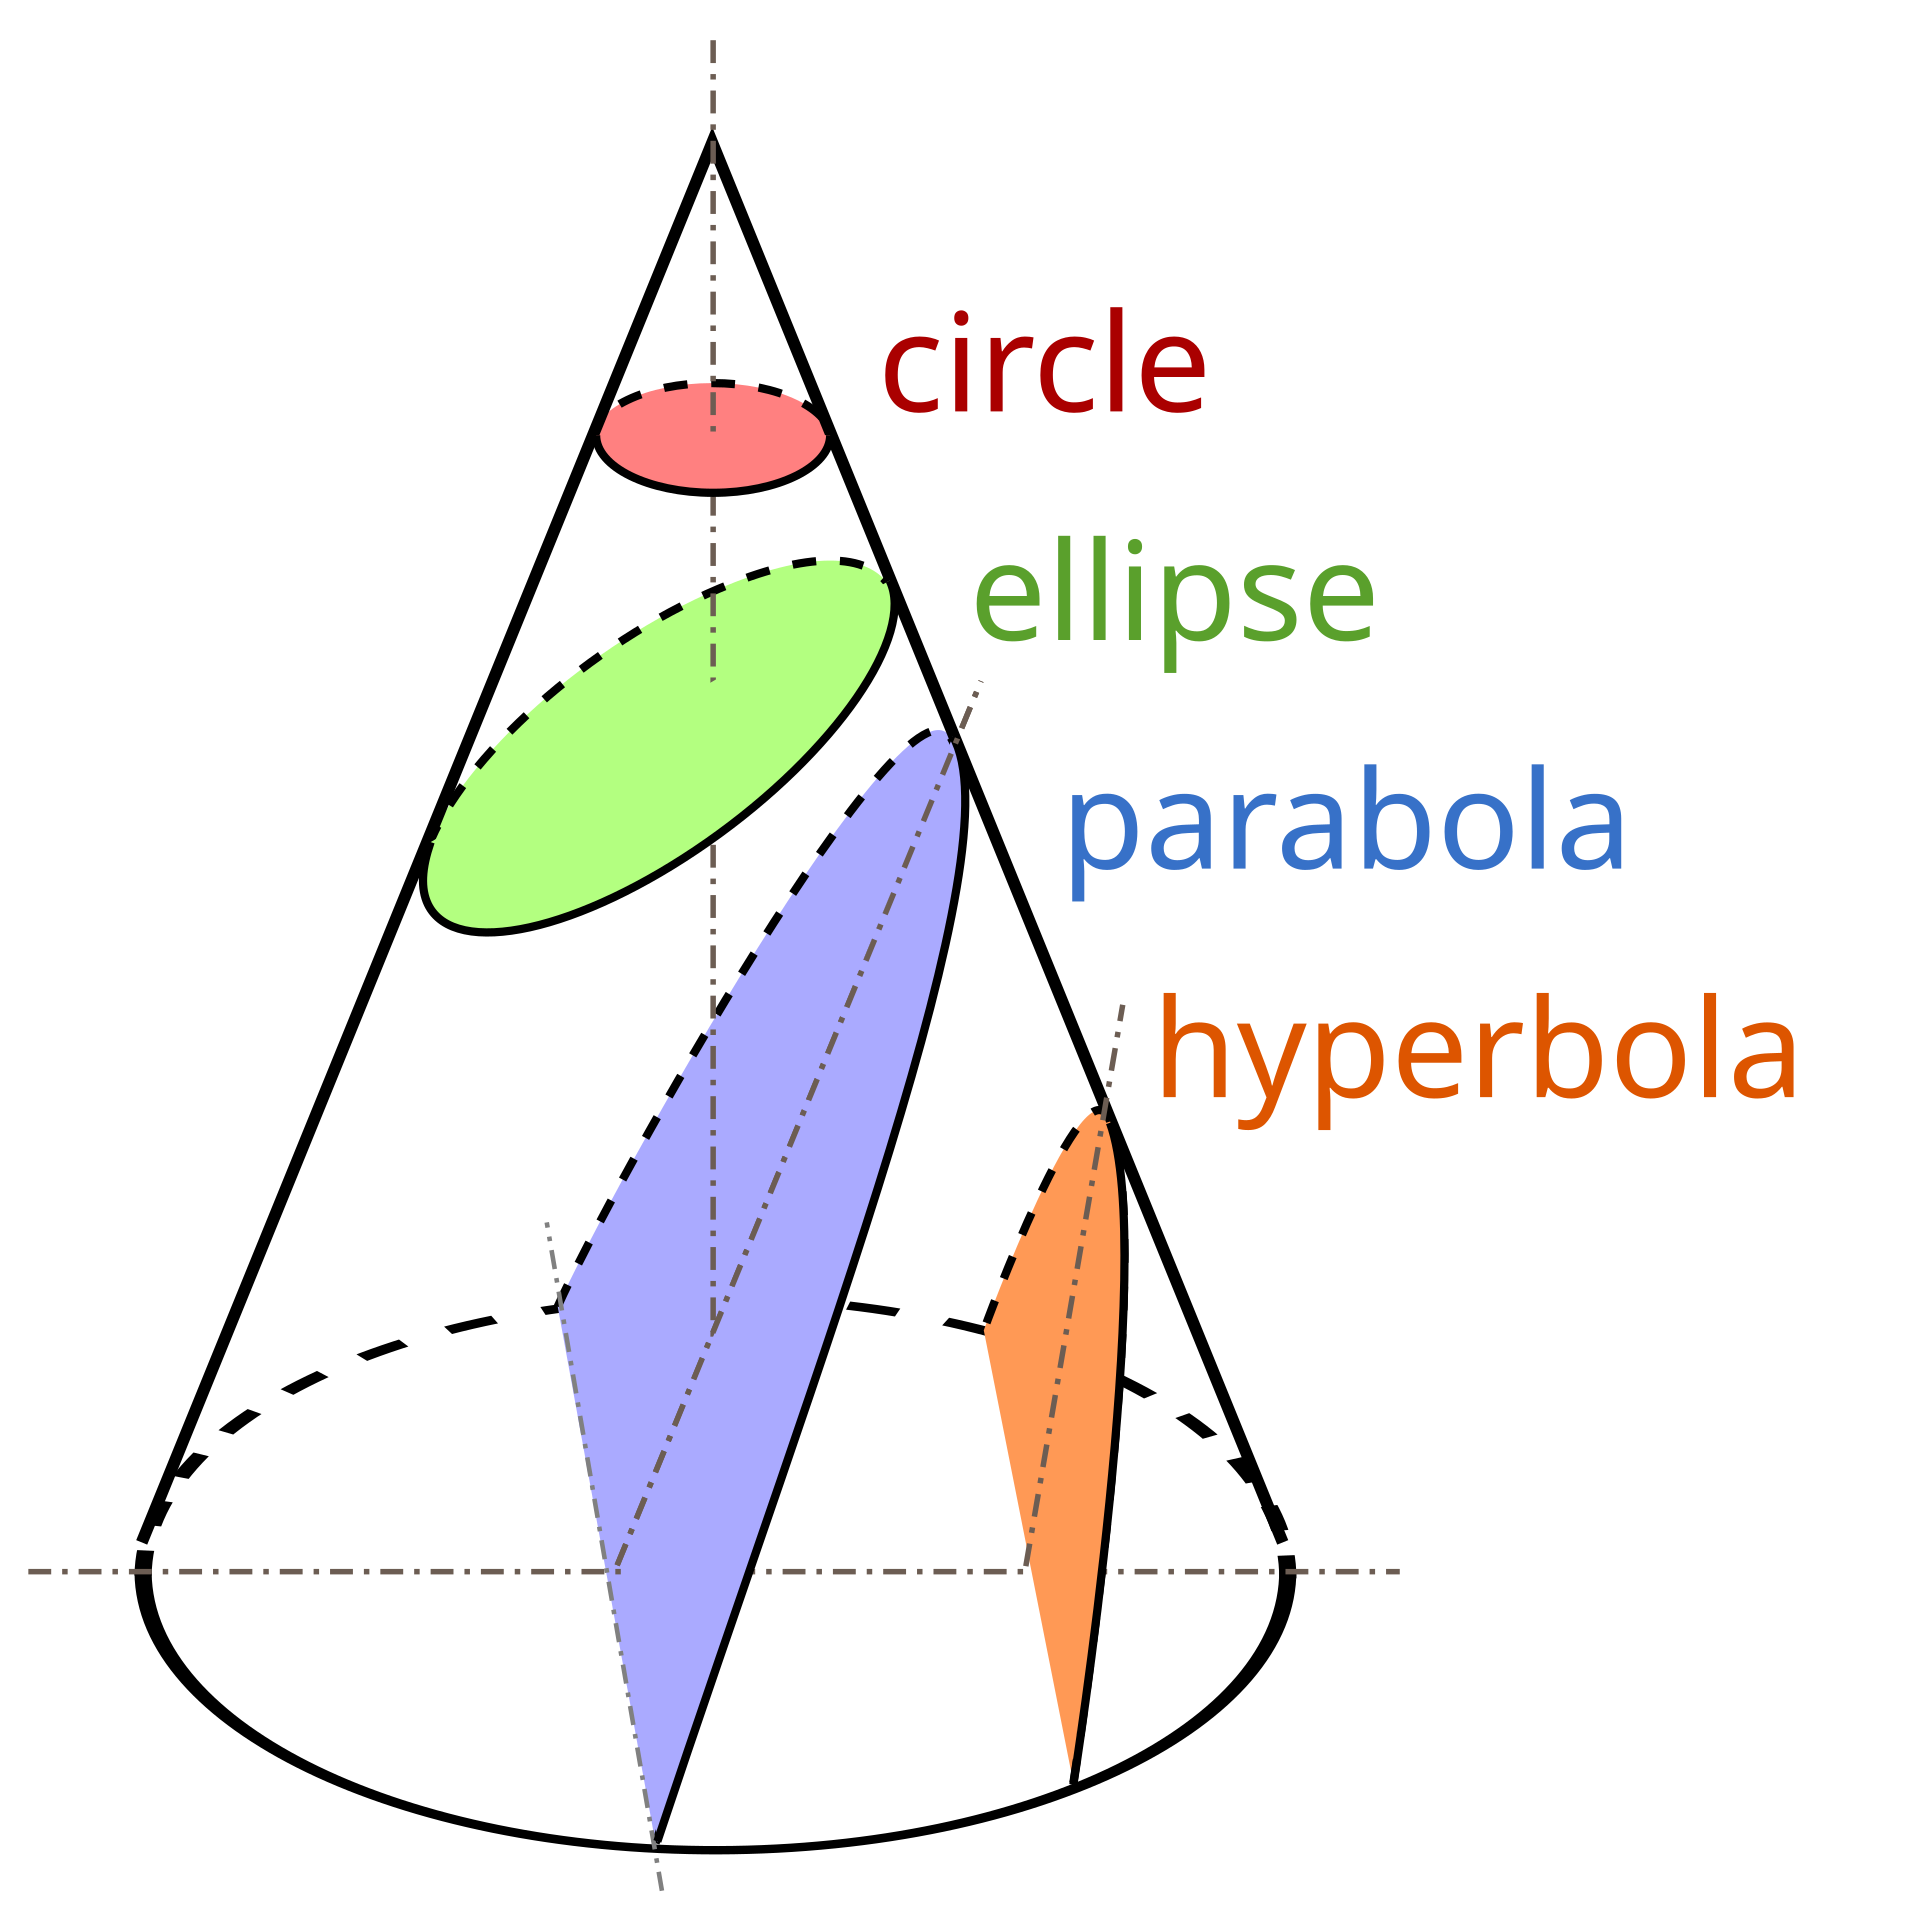
\includegraphics[width=7cm]{Conic_Sections.png}
  \caption{Visualization of conic sections.}
  \caption*{\small Source: Wikimedia Commons, Public Domain: \url{https://upload.wikimedia.org/wikipedia/commons/thumb/1/11/Conic_Sections.svg/1920px-Conic_Sections.svg.png}}
\end{figure}

% the diagram on the thumbnail of this could be replicated:
% https://youtu.be/PLrgwD9TleU?si=7I_kDFHFqqPIHtSo

\section{Definitions}

Each type of conic sections can be defined as follows:

\subsection{Circle}

A circle is the set of all points in a plane that are at a given
distance (the radius) from a given point (the center). The standard
equation for a circle with center $(h,k)$ and radius $r$ is:

\begin{equation}
(x - h)^2 + (y - k)^2 = r^2
\end{equation}

\begin{center}
  
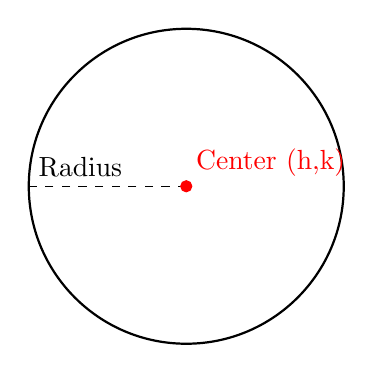
\begin{tikzpicture}
  \draw[thick] (0,0) circle (2cm);
  
  % \draw[dashed] (-4,0) -- (4,0) node[anchor=west] {Major Axis};
  \draw[dashed] (0,0) -- (-2,0) node[above right] {Radius};

  \filldraw[red] (0,0) circle (2pt) node[above right] {Center (h,k)};


\end{tikzpicture}
\end{center}


\subsection{Ellipse}

An ellipse is the set of all points such that the sum of the distances
from two fixed points (the foci) is constant. The standard equation
for an ellipse centered at the origin with semi-major axis $a$ and
semi-minor axis $b$ is:

\begin{equation}
\frac{x^2}{a^2} + \frac{y^2}{b^2} = 1
\end{equation}

\begin{center}
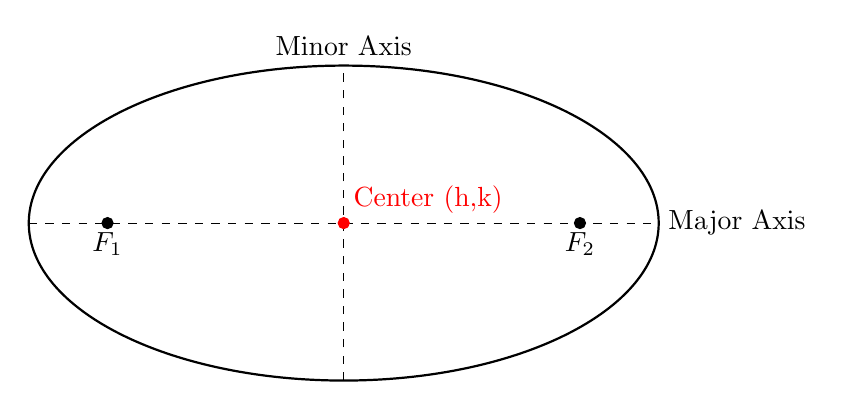
\begin{tikzpicture}
  \draw[thick] (0,0) ellipse (4cm and 2cm);
  
  \draw[dashed] (-4,0) -- (4,0) node[anchor=west] {Major Axis};
  \draw[dashed] (0,-2) -- (0,2) node[anchor=south] {Minor Axis};

  \filldraw[black] (-3,0) circle (2pt) node[below] {$F_1$};
  \filldraw[black] (3,0) circle (2pt) node[below] {$F_2$};

  \filldraw[red] (0,0) circle (2pt) node[above right] {Center (h,k)};


\end{tikzpicture}
\end{center}
\subsection{Hyperbola}

A hyperbola is the set of all points such that the absolute difference
of the distances from two fixed points (the foci) is constant. A hyperbola is formed from slicing a \emph{double-cone} --- two cones placed tip-to-tip --- parallel to or angled off of the central axes.  The
standard equation for a hyperbola centered at the origin is:

\begin{equation}
\frac{x^2}{a^2} - \frac{y^2}{b^2} = 1
\end{equation}

or

\begin{equation}
\frac{y^2}{b^2} - \frac{x^2}{a^2} = 1
\end{equation}

depending on the orientation of the hyperbola.

%FIXME diagram


\subsection{Parabola}

A parabola is the set of all points that are equidistant from a fixed
point (the focus) and a fixed line (the directrix). The standard
equation for a parabola that opens upwards or downwards is:

\begin{equation}
y = a(x - h)^2 + k
\end{equation}

and that opens leftwards or rightwards is:

\begin{equation}
x = a(y - k)^2 + h
\end{equation}

\begin{center}
  
\begin{tikzpicture}
  \draw[thick] (0,0) parabola (4,4);
  \draw[thick] (0,0) parabola (-4,4);
  

  \filldraw[red] (0,0) circle (2pt) node[below] {Center (h,k)};


\end{tikzpicture}
\end{center}


where $(h,k)$ is the vertex of the parabola, and $a$ is a scalar.

Note that only the parabola out of these four is a function, as passes vertical line test. The other three cannot be expressed as functions, only equations.
% talk about asymptotes in this chaptter